\documentclass[anchorcolor=blue,linkcolor=blue]{beamer}
\usepackage{booktabs}
\usepackage{amsmath}
\usepackage{xcolor}
  
\hypersetup{colorlinks,linkcolor=,urlcolor=blue}

%%\usepackage{blkarray}
\mode<presentation>
{
%  \usetheme{Malmoe}
\usetheme{default}
%\usecolortheme{seahorse}
  % or ...

% \setbeamercovered{transparent}
  % or whatever (possibly just delete it)
% \setbeamertemplate{footline}[default]
% \setbeamertemplate{navigation symbols}{\insertslidenavigationsymbol\insertframenavigationsymbol\insertdocnavigationsymbol}
}
\usepackage[english]{babel}

\title{How many (rare) diseases are there?}
\subtitle{A feeble attempt at systematic disease\\
  harmonization across ontologies} 
\author{Dac-Trung Nguyen\and Qian Zhu\\[1em] \emph{NCATS Informatics}}
\date{{\Large$\pi\!$}, 2019}

\begin{document}

\begin{frame}
  \titlepage
\end{frame}

\begin{frame}
  \begin{block}{How dare you?}
    \begin{itemize}
    \item No agreed upon definition for what a ``disease'' is
    \item \emph{disease} $\rightleftharpoons$ \emph{syndrome}
      $\rightleftharpoons$ \emph{condition} $\rightleftharpoons$
      \emph{indication} $\cdots$
    \item Numerous ontologies: MeSH, OMIM, Disease Ontology, Orphanet,
      GARD, UMLS, HPO, MONDO, $\ldots$
    \item Entity resolution/normalization and ontology matching are
      still unsolved problems
    \end{itemize}
  \end{block}
  \begin{block}{Baby steps...}
    \begin{enumerate}
      \item Build a comprehensive knowledge graph based on available
        ontologies: \href{https://www.ebi.ac.uk/ols/ontologies}{Ontology
          Lookup Service}
      \item Build on our previous effort for
        \href{https://stitcher.ncats.io/app/stitches/latest}{drug harmonization} using
        in-house
        \href{https://spotlite.nih.gov/ncats/stitcher.git}{stitcher} codebase
      \item Focus on the GARD subset
    \end{enumerate}
  \end{block}
\end{frame}

\begin{frame}
  \frametitle{Disease knowledge graph}
  \begin{itemize}
  \item Available as a Neo4j database at
    
    \centerline{\href{https://disease.ncats.io/browser}{\texttt{https://disease.ncats.io/browser}}}
    \begin{itemize}
    \item No username/password required
    \item Use \texttt{disease.ncats.io:7687} as the \textbf{Host}
    \end{itemize}
  \item Based on the following data sources:
    \begin{center}
      \tiny
      \begin{tabular}{rl}\toprule
        Data Source & Entities\\ \midrule
        \texttt{GARD\_v1}&6763\\
        \texttt{BrendaTissue.owl.gz}&5902\\
        \texttt{GHR\_v1}&1287\\
        \texttt{DOID.owl.gz}&12694\\
        \texttt{HPO.owl.gz}&17387\\
        \texttt{MEDLINEPLUS.ttl.gz}&2238\\
        \texttt{MESH.ttl.gz}&275329\\
        \texttt{MONDO.owl.gz}&110363\\
        \texttt{OMIM.ttl.gz}&102715\\
        \texttt{UBERON.owl.gz}&15909\\
        \texttt{ordo.owl.gz}&13871\\
        \texttt{GO.owl.gz}&49290\\
        \texttt{ogg.owl.gz}&69688\\
        \texttt{pr.owl.gz}&315937\\
        \texttt{ogms.owl}&91\\
        \texttt{pato.owl.gz}&2730\\
        \texttt{chebi.xrdf.gz}&130403\\
        \texttt{FDAOrphanGARD\_20190216.txt}&6074\\
        \texttt{rancho-disease-drug\_2018-12-18\_13-30.txt}&19817\\
        \texttt{HPO\_annotation\_100918.txt}&164448\\ \bottomrule
      \end{tabular}
    \end{center}
  \end{itemize}
\end{frame}

\begin{frame}
  \frametitle{A closer look at GARD}
    
  \begin{block}{GARD diseases by content feature}
    \begin{center}
      \begin{tabular}{cc}\toprule
        Content Feature & Count\\ \midrule
        Prevalence & 95 \\
        Diagnosis & 577\\
        Inheritance & 702\\
        Treatment & 1037\\
        Cause & 873\\
        Symptoms & 835\\
        Prognosis & 568\\ \bottomrule
      \end{tabular}
    \end{center}
    Total 6,763 diseases, of which 6,504 are considered rare. Out of
    6,504 rare diseases, there are 480 that do not map to anything (e.g.,
    \emph{Hillig syndrome}). It turns out that about 58 of these do map
    to UMLS exactly; e.g., \emph{Webster Deming syndrome} (GARD 428)
    maps to \emph{Craniofrontonasal dysplasia with Poland anomaly
      syndrome} (C4303859).
  \end{block}
\end{frame}

\begin{frame}
  \frametitle{GARD disease categories}
  \begin{center}
    \tiny
    \begin{tabular}{rl}\toprule
      Category & Count\\ \midrule
      Congenital and Genetic Diseases&3040\\
      Nervous System Diseases&1254\\
      Musculoskeletal Diseases&652\\
      Skin Diseases&591\\
      Eye diseases&573\\
      Rare Cancers&532\\
      Metabolic disorders&509\\
      Blood Diseases&321\\
      Kidney and Urinary Diseases&290\\
      Endocrine Diseases&263\\
      Digestive Diseases&248\\
      Ear, Nose, and Throat Diseases&242\\
      Mouth Diseases&210\\
      Heart Diseases&176\\
      Chromosome Disorders&151\\
      Immune System Diseases&148\\
      Lung Diseases&137\\
      Female Reproductive Diseases&89\\
      Newborn Screening&84\\
      Male Reproductive Diseases&70\\
      Bacterial infections&58\\
      Viral infections&39\\
      Parasitic diseases&33\\
      Hereditary Cancer Syndromes&26\\
      Connective tissue diseases&22\\
      Fungal infections&12\\
      Autoimmune / Autoinflammatory diseases&9\\
      Behavioral and mental disorders&7\\
      Nutritional diseases&3\\
      Environmental Diseases&2        \\ \bottomrule
    \end{tabular}
  \end{center}
\end{frame}

\begin{frame}
  \frametitle{Disease resources}
  \begin{center}
    \begin{tabular}{rl}
      GARD &
      \href{https://rarediseases.info.nih.gov/}{\texttt{https://rarediseases.info.nih.gov/}}\\
      Orphanet &
      \href{https://www.orpha.net}{\texttt{https://www.orpha.net}}\\
      GHR&
      \href{https://ghr.nlm.nih.gov/}{\texttt{https://ghr.nlm.nih.gov/}}\\
      Disease Ontology (DO) &
      \href{http://disease-ontology.org/}{\texttt{http://disease-ontology.org/}}\\
      OMIM & \href{https://omim.org/}{\texttt{https://omim.org/}}\\
      MeSH &
      \href{https://meshb.nlm.nih.gov}{\texttt{https://meshb.nlm.nih.gov}}\\
      MEDLINE+ &
      \href{https://medlineplus.gov/}{\texttt{https://medlineplus.gov/}}\\
      MONDO &
      \href{http://monarchinitiative.org/}{\texttt{http://monarchinitiative.org/}}\\
      HPO & \href{https://hpo.jax.org}{\texttt{https://hpo.jax.org}}\\
    \end{tabular}
  \end{center}
\end{frame}

\begin{frame}
  \frametitle{Disease overlap matrix}
  \begin{block}{Direct match by synonyms or identifiers}
    \begin{center}
      \tiny
      \begin{tabular}{rccccccccc}\toprule
        & GARD & Orphanet & GHR & DO & OMIM & MeSH & MEDLINE+&MONDO & HPO\\ \midrule
        GARD & \textbf{6,504}&4,377&837&2,760&3,597&4,017&257&5,796&715\\
        Orphanet &4,299&\textbf{9,290}&616&3,301&4,427&3,613&280&8,973&858\\
        GHR &829&616&\textbf{1,287}&620&556&876&99&1,125&143\\
        DO &2,506&3,554&617&\textbf{8,699}&3,473&3,295&722&8,679&1,502\\
        OMIM &4,850&7,313&883&5,842&\textbf{12,883}&8,505&664&11,374&2,491\\
        MeSH &3,889&3,330&836&3,140&5,871&\textbf{8,892}&653&7,882&1,153\\
        MEDLINE+ &310&414&99&966&495&743&\textbf{2,238}&662&440\\
        MONDO &6,573&11,856&1,245&10,776&8,696&8,555&645&\textbf{21,826}&2,385\\
        HPO &730&868&143&1,510&1,458&1,382&379&2,237&\textbf{13,725}\\ \bottomrule
      \end{tabular}
    \end{center}
    The matrix is asymmetric due to $1-n$ and/or $m-1$ mappings; e.g.,
    there are $4,377$ GARD diseases that mapped to $4,299$ diseases in
    Orphanet. These numbers improve as we extend the
    matching indirectly to two-, three-, four-neighbor. 
  \end{block}
\end{frame}

\begin{frame}
  \frametitle{Disease harmonization challenges}
  \begin{block}{How many ``distinct'' diseases are here?}
    \centerline{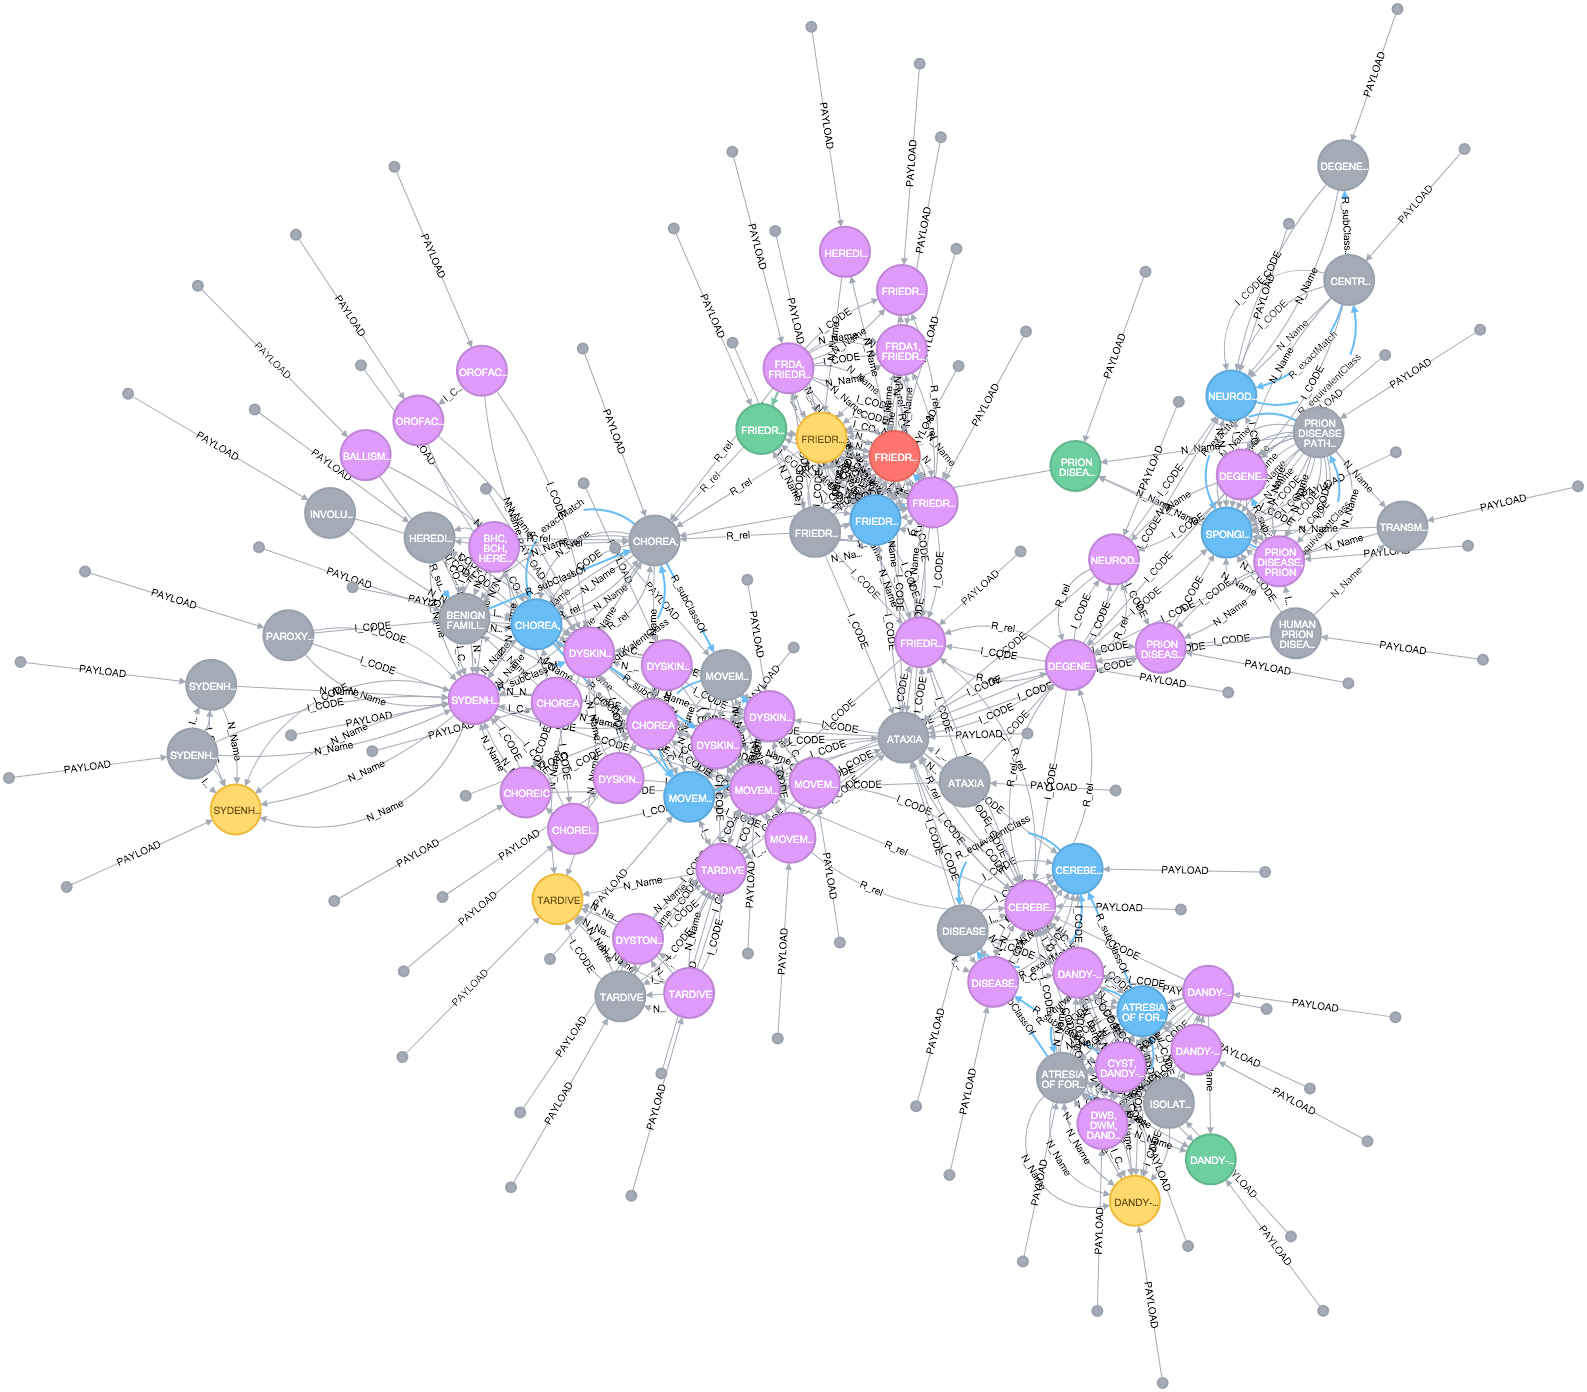
\includegraphics[width=9cm]{graph1}}
  \end{block}
\end{frame}

\begin{frame}
  \frametitle{A strategy for harmonization}
  \begin{enumerate}
  \item Generate \emph{strongly connected components}
    \begin{itemize}
    \item Perform transitive closure on nearest (weighted) neighbors
    \end{itemize}
  \item For each strongly connected component, do the following:
    \begin{enumerate}
    \item Calculate pair-wise similarities for all synonyms and
      identifiers based on Jaccard metric \[\text{sim}(x,y) =
      \frac{|x\cap y|}{|x\cup y|}\]
    \item Group synonyms and identifiers based on $\text{sim}(x,y) \ge
      \delta$ ($\delta=0.4$ gives reasonable grouping)
    \item Each such synonym/identifier grouping serves as an initial
      seed for which entities are then merged/split
    \end{enumerate}
  \end{enumerate}
\end{frame}

\begin{frame}
  \frametitle{Next steps}
  \begin{enumerate}
  \item Ongoing evaluation of the proposed harmonization strategy
  \item How best to normalize entities?
    \begin{itemize}
    \item Identify preferred synonyms and identifiers
    \end{itemize}
  \item Support manual curation and harmonization cycle
  \end{enumerate}
\end{frame}

\begin{frame}[fragile]
  \frametitle{Example cypher queries on disease knowlege graph}
  \begin{block}{Data source listing}
    \small
\begin{verbatim}
match(n:DATASOURCE) return n.name,n.instances
\end{verbatim}
  \end{block}

  \begin{block}{OMIM disease count}
    \small
\begin{verbatim}
match(n:`OMIM.ttl.gz`:T047) return count(n)
\end{verbatim}
  \end{block}
  
  \begin{block}{GARD disease category breakdown}
    \small
\begin{verbatim}
match(n:`GARD_v1`)-[]-(m:DATA) where m.is_rare=true 
with distinct labels(n) as t, count(n) as cnt 
unwind  t as Category
return Category,sum(cnt) as Count order by Count desc
\end{verbatim}
  \end{block}
\end{frame}

\begin{frame}[fragile]
  \frametitle{Example of overlap query}
  \begin{block}{Orphanet and MONDO}
    \small
\begin{verbatim}
match(n:`ordo.owl.gz`)-[]-(m:DATA) 
where not exists(m.symbol) 
and not exists(m.reason_for_obsolescence) 
with n match(n)-[:N_Name|
   :I_CODE*1]-(a:`MONDO.owl.gz`)-[]-(b:DATA) 
where exists(b.label) and not exists(a.status) 
return count(distinct n) as `Orphanet`,
    count(distinct a) as `MONDO`
\end{verbatim}
  \end{block}
\end{frame}
\end{document}
